\documentclass[a4paper, 11pt]{scrartcl}
\usepackage{fullpage}
\usepackage{graphicx}
\usepackage{appendix}
\usepackage{booktabs}

% hyperref and nameref so that we can have sane internal refs
% hyperref also helps with pdf index creation
\usepackage[linkcolor={blue},citecolor={blue},urlcolor={red}]{hyperref}
\usepackage{nameref}

% Place all of the figures at the end of the document
\usepackage[figuresonly,nomarkers,nolists]{endfloat}
\renewcommand{\efloatseparator}{}

% Set to false for black/white printing
\hypersetup{colorlinks=true}

\title {Student Robotics 2013\\ Rulebook}
\author{Revision 6}
\date{\today}
\setcounter{tocdepth}{1}

\begin {document}
\maketitle

\noindent The following defines the rules and regulations of the Student Robotics 2013 competition.

\newcounter{rule}[section]
\newcommand{\rcn}{\stepcounter{rule}\arabic{section}.\arabic{rule}}
\renewcommand{\labelenumi}{\rcn}

\section {Game Rules}
\label{game-rules}

\begin{enumerate}
\item The game, called \textbf{A Strange Game}, will be played in the arena defined in section~\ref{sub:arena}.
      The objective of this game is to achieve as many points as possible by placing your tokens on squares and pedestals to capture them.

\item Before a match begins, participating teams must:
\begin {enumerate}
  \item Present their robot in the staging area, adjacent to the arena, at least 2 minutes before the scheduled start time.
        The staging area will be clearly marked on the day.

  \item Attach four robot badges.
        These badges will be provided by Student Robotics officials in the staging area.
        Section~\ref{sec:robot-badges} provides more information about these badges, as well as their dimensions and mounting requirements.

  \item Place their robot in the starting zone that they are assigned.
        The robot must be placed such that it is entirely within this starting zone, with no parts overhanging its boundary.

  \item Place a single token in/on their robot if they so wish.

  \item Vacate the arena 40 seconds before the scheduled start time.
        During the 40 second period prior to the start of the match there must be no interaction with the robot.
\end{enumerate}
  Teams that fail to comply with this rule may forfeit the match, at the discretion of the judge.

\item A match lasts 180 seconds.

\item There will be a maximum of 4 robots in a match.

\item At the end of a match, each team's ``\textbf{game points}'' will be calculated.
      These are used to rank teams before competition league points are awarded.
      Game points will be awarded as follows:
\begin{enumerate}
  \item \textbf{1 point} will be awarded for initial movement outside the starting zone, defined as when the back of the robot passes over the boundary.
  \item For each row of squares, \textbf{1 point} will be awarded if one square is captured, \textbf{3 points} will be awarded if two squares are captured, and \textbf{6 points} will be awarded if all squares are captured.
  \item For each column of squares, \textbf{1 point} will be awarded if one square is captured, \textbf{3 points} will be awarded if two squares are captured, and \textbf{6 points} will be awarded if all squares are captured.
  \item At the end of the round, points will be clamped to zero if negative.

      See figure \ref{fig:scoring} for an example on how scores are calculated.

\begin{figure}
  \centering
  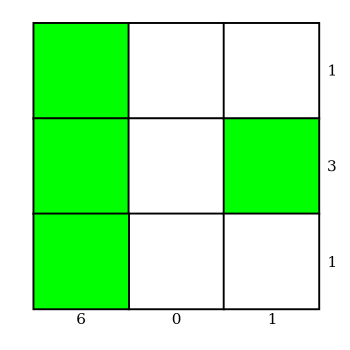
\includegraphics{./images/scoring.pdf}
  \caption{If a robot were to finish the match in control of the green squares above, then they would receive 1 point from the north row, 3 points from the centre row, 1 point from the south row, 6 points from the west column, 0 points from the centre column, and 1 point from the east column, leading to a total of 12 points from square control. We are aware that this is different from what was stated at Kickstart, and apologise for this.}
  \label{fig:scoring}
\end{figure}
\end{enumerate}

\item Ownership of a square will be determined as follows:
\begin{enumerate}
  \item If there are one or more tokens on the central pedestal, the square will be deemed to have been captured by the robot associated with the highest token in the stack.
  \item Otherwise, if one robot has more tokens in the square than any other, that robot is deemed to have captured the square.
  \item Otherwise, the square is deemed unclaimed.
  \item A token is deemed to be in a square if the majority of the token is within the inner edge of the line delineating the square. The judges decision is final.
\end{enumerate}

\item At the end of a game, league points will be awarded as follows.
      The team with the \emph{most} game points will be awarded 4 points towards the competition league.
      The team with the second most will be awarded 3.
      The team with the third most will be awarded 2 points, and the team with the fewest game points will be awarded 1 point.
      Teams whose robot was not entered into the round, or who were disqualified from the round, will be awarded no points.

      Tied robots will be awarded the average of the points that their combined positions would be awarded.
      Thus, three robots tied for first place would receive 3 points each (since this is $(4+3+2)/3$).

\item Once the league has completed, a knockout competition will begin.
      The positions of the teams in the league will seed the positions of teams in the knockout matches.
      The top 24 teams from the league advance to the knockout.
      In the event of tied league positions, the team with the greatest cumulative game points in the league will go through.

      Each match in the knockout competition involves up to 4 teams.
      The teams that come 1\textsuperscript{st} and 2\textsuperscript{nd} in each knockout match will continue to the next round of the knockout.
      In the event of a tie in a knockout match, the team that ranked highest in the league will go through.
      If there is a tie in the final, then a rematch will be played.
      The number of league and knockout matches will be announced on the morning of the competition.

\item Robots will be started by teams leaning into the arena to press the start button on their robot\footnote{A wireless match-starting solution may be provided by Student Robotics.} when instructed to do so.


\item A match may be terminated prematurely if all teams participating in that match state to the judge that they are happy for the game to end.

\item A token will be considered to be on a pedestal if the token is fully supported by the pedestal, and no part of the token is in contact with a robot, or any other part of the arena.

\end{enumerate}

\newpage
\section {Regulations}
\label{sec:Regulations}

\begin{enumerate}

%% Behaviour

\item No remote control systems may be used.
\item This is a non-contact sport, but accidental bumps and scrapes are inevitable.
\item Robots must not intentionally damage anything -- including tokens, pedestals, the arena or other robots.
      At the discretion of the judge, teams who deliberately engage in collisions or take insufficient precautions against collisions may be penalised, including disqualification from rounds and deduction of league points.
\item Student Robotics reserves the right to examine your robot software and hardware at any time.
\item Assistance from Student Robotics Engineers is provided without any guarantees.
\item All kit deployed by Student Robotics remains the property of Student Robotics.
      All electronic kit \textbf{must} be returned to Student Robotics after the competition.
      \autoref{sec:kit-return} details the parts of the kit that must be returned.
      After the competition, the kit that is not specified in \autoref{sec:kit-return} becomes the property of the team.

\item The Judge's decision is final.

%% Physical

\item Robots must pass an inspection by a Student Robotics Inspector before competing in a match.
      This inspector will check that the robot complies with the rules and regulations of this game, and is safe to compete (see \autoref{sec:safety-regs}).
      \textbf{Robots that have not passed inspection will not be permitted to compete}.

\item At the beginning of each match, robots must fit within a cube with $500mm$ internal sides.
      \textit{During the match}, the robot may extend beyond this size.
      This only includes the size of the robot and not a token which may optionally be placed in or on the robot before the start of the match.

\item The power board, including its power switch, must be easily accessible at all times -- including throughout the game.
      This is for everyone's safety, especially your robot's.

\item All custom electronics that require a connection to the battery must instead be connected to the motor rail.
      There are extra connectors on the power board for this purpose.

\item All wires connected to the robot's ground (0V line) must be black.
      Black wires \emph{must not} be used for anything else.
      It is \emph{strongly recommended} that all wiring is neat and easily removable, as this will reduce the time required to debug problems on robots
       (teams may be asked to tidy their wiring before a Student Robotics Engineer will approach any issues with their robot).

\item All electronics must be securely fixed to the robot, and should also be easily removable.

\item It must not be possible to injure oneself on the robot.
      This will be tested using a Frankfurter sausage to simulate a finger.
      For example, high-speed rotating parts that could cause injury must be suitably shielded.

\item Robots must feature four mountings for robot badges.
      These mountings must comply with the specification in section~\ref{sec:robot-badges}.

\item The lithium-ion polymer batteries provided in the kit must be shielded from mechanical and thermal harm.
      This includes mechanical protection from accidental impact with other robots.
      Teams found to be in violation of this rule will have their batteries confiscated until they have demonstrably rectified the identified issues.

\item If teams wish to use batteries other than the lithium-ion polymer batteries provided,
       then they must seek approval from Student Robotics through the Student Robotics forums first.
      Additionally, if teams wish to add systems powered by separate batteries then they must seek approval through the same channel first.

      In general, teams are encouraged to power everything off the SR-supplied battery through the power board.
      All electromechanical components \textbf{must} be powered through the motor rail provided by the power board.

\item Robots may not include radio transmitters or receivers.
      In exceptional circumstances, teams may request an exemption from this rule.

\end{enumerate}

\newpage
\section{Specifications}
\label{sec:Specifications}

\newcounter{rulei}[subsection]
\newcommand{\rcnii}{\stepcounter{rulei}\arabic{section}.\arabic{subsection}.\arabic{rulei}}
\renewcommand{\labelenumi}{\rcnii}

\subsection{Markers}
\label{sub:markers}
The arena, tokens, pedestals, and robots involved in the game are labelled with \textit{libkoki} markers.
Each marker pattern encodes a number.
Each marker number is associated with a particular feature within the arena, and also has an associated size.
The marker numbers and sizes are as follows:

\begin{center}
  \begin{tabular}{lcc}
    \toprule
    \textbf{Item} & \textbf{Marker Numbers} & \textbf{Marker Size (mm)} \\
    \midrule
    Arena boundary & 0 -- 27 & 250 \\
    Robots & 28 -- 31 & 100 \\
    Pedestals & 32 -- 40 & 200 \\
    Tokens & 41 -- 64 & 200 \\
    \bottomrule
  \end{tabular}
\end{center}

Two sets of marker codes will be used: one for development purpose, and one for the competition itself.
The competition set is only to be used inside the Student Robotics arena at the Student Robotics competition.
This is so that people carrying markers past the arena do not confuse robots.
The competition codes are 100 above the development codes.
When run in competition mode (specifiable through the robot's GUI), the software provided by Student Robotics will subtract 100 from the detected marker codes, as well as ignore the development codes.

The markers can be printed on a black-and-white printer.
Marker designs can be downloaded from the documentation section of the Student Robotics website.

Unless specified otherwise, all markers described in this document are oriented vertically such that the principle corner of the marker (which is indicated by a dark grey dot in the black marker border) is on the higher edge.

\subsection{Robot Badges}
\label{sec:robot-badges}

\begin{figure}
  \centering
  \includegraphics[width=\textwidth]{./images/robot-marker.pdf}
  \caption{An example robot badge.
           The blue areas shown are the human-compatible areas.
           All dimensions are in millimetres.}
  \label{fig:example-badge}
\end{figure}

\begin{enumerate}
\item A ``robot badge'' is a removable identifier that will be attached to a robot throughout a match.
      It features the robot's assigned marker for the match, as well as human-compatible areas to allow spectators to easily associate a robot with its starting location.
      An example of one of these badges is shown in figure~\ref{fig:example-badge}.
      The markings in the human-compatible areas are intentionally not specified.

\item A robot must feature four of the badge mounts shown in figure~\ref{fig:badge-mounting}.
      These mounts must permit a flat $200 \times 100mm$ panel to be attached to them.
      The three areas of each mount must feature the illustrated areas of hook-type Velcro to allow this panel to be fitted.

\item The four badge mounts must be on the exterior of the robot, parallel with the vertical plane, and should be perpendicular to each other about the vertical axis\footnote{Teams can apply for a team-specific rule alteration to the required number of badges.
      Clear justification must be provided by the team with such a request.}
      The orientation of the badge mounts is unimportant, but teams are encouraged to position them horizontally as shown in figure~\ref{fig:example-badge}.

\item The mapping between a given robot and its robot badge is as follows:

\begin{center}
  \begin{tabular}{cc}
    \toprule
    \textbf{Zone} & \textbf{Marker Number} \\
    \midrule
    0 (NW) & 28 \\
    1 (NE) & 29 \\
    2 (SE) & 30 \\
    3 (SW) & 31 \\
    \bottomrule
  \end{tabular}
\end{center}

\begin{figure}
  \centering
  \includegraphics[width=\textwidth]{./images/badge-mounting.pdf}
  \caption{The dimensions of the required robot badge mountings.
           The shaded areas are hook-type Velcro.
           All dimensions are in millimetres.}
  \label{fig:badge-mounting}
\end{figure}

\end{enumerate}

\subsection{Arena}
\label{sub:arena}
\begin{enumerate}
\item The match arena floor, overall, is an $8m \times 8m$ square, as shown in figure~\ref{fig:arena-dim}.
      The tolerance of these two dimensions is $\pm0.25m$.

\begin{figure}
  \centering
  \includegraphics[width=\textwidth]{./images/arena.pdf}
  \caption{\label{fig:arena-dim}A bird's-eye view of the arena.}
\end{figure}

\item The floor of the arena is carpeted with blue carpet tiles.
      The carpet tiles used in the arena are from B\&Q, with EAN 5014957151543.

\item The arena walls are $600\pm30mm$ high, the interior surfaces of which are white plastic-coated hardboard.

\item The arena features nine \textit{squares}.
      These areas are delineated by lines marked on the arena floor with $25mm$ wide paper-based masking tape.
      The naming of these squares is shown in figure~\ref{fig:arena-dim}.

\begin{figure}
  \centering
  \includegraphics[width=\textwidth]{./images/sidewall.pdf}
  \caption{Seven $250mm$ wide markers are spaced evenly along each $8m$ arena wall.
           The markers are placed $50mm$ above the floor.
	   All dimensions are in millimetres.}
  \label{fig:arena-wall}
\end{figure}

\begin{figure}
  \centering
  \includegraphics[width=0.5\textwidth]{./images/arena-markers.pdf}
  \caption{Twenty eight arena wall markers are positioned around the perimeter of the arena with the marker codes incrementing in an anti-clockwise fashion from the northern end of the west wall.
           The zones are counted from the north west corner in a clockwise fashion.}
  \label{fig:arena-zones}
\end{figure}

\item Each wall of the arena features seven $250mm$ libkoki markers.
      Figure~\ref{fig:arena-wall} shows the positioning of these markers, whilst figure~\ref{fig:arena-zones} shows the numbering of these markers.

\item Each robot will be assigned a zone number at the start of every match to indicate its starting position.
      The mapping of these zone numbers in the arena is shown in figure~\ref{fig:arena-zones}.

\item Student Robotics reserves the right to have up to three match officials in the arena during games.

\end{enumerate}

\subsection{Pedestals}
\label{sub:pedestals}
\begin{enumerate}
\item Pedestals are cuboid structures with base $320 \times 320mm \pm 15mm$.
      The top of a pedestal has a $20mm \pm 5mm$ high rim to prevent tokens falling off.
      The height of the pedestal, including the rim is $340mm \pm 15mm$.

\item Pedestals will be securely attached to the floor of the arena to prevent them being moved.

\item Each pedestal features a $200mm$ marker in the centre of each vertical side.

\item The mapping between pedestal position and marker is as follows:

\begin{center}
  \begin{tabular}{cc}
    \toprule
    \textbf{Position} & \textbf{Marker Number} \\
    \midrule
    NW & 32 \\
    N  & 33 \\
    NE & 34 \\
    W  & 35 \\
    C  & 36 \\
    E  & 37 \\
    SW & 38 \\
    S  & 39 \\
    SE & 40 \\
    \bottomrule
  \end{tabular}
\end{center}

\end{enumerate}

\subsection{Tokens}
\label{sub:Tokens}
\begin{enumerate}
\item Tokens are cubic corrugated cardboard boxes with side $305 \pm 15 mm$.
      \emph{Each team's kit contains two of these.}

\item Each token is associated with its own libkoki marker number and is labelled with six identical $200mm$ markers -- one on each face.

\item Tokens will be styled to match the human-compatible area of the robot badges on their associated robot, allowing spectators to follow game play.
      See section~\ref{sec:robot-badges}.

\item The mapping between a given robot and its tokens is as follows:

\begin{center}
  \begin{tabular}{cc}
    \toprule
    \textbf{Zone} & \textbf{Marker Numbers} \\
    \midrule
    0 (NW) & 41 -- 46 \\
    1 (NE) & 47 -- 52 \\
    2 (SE) & 53 -- 58 \\
    3 (SW) & 59 -- 64 \\
    \bottomrule
  \end{tabular}
\end{center}

\item The tokens belonging to a given robot will initially be positioned to the left of the robot as shown in figure~\ref{fig:token-position}.
      Teams have the option to place any one of their six tokens in/on their robot before the start of the match.

\begin{figure}
  \centering
  \includegraphics[width=\textwidth]{./images/token-position.pdf}
  \caption{Six $305 \pm 15mm$ wide tokens are spaced evenly $300 \pm 20mm$ to the left of the robot, along the arena wall.
           The tokens are placed $100 \pm 20mm$ away from each other and the edge of the arena.
           All dimensions are in millimetres.}
  \label{fig:token-position}
\end{figure}

\end{enumerate}

\clearpage

\newpage
\input {awards}

\renewcommand{\labelenumi}{\rcn}

\section{Clarifications}
Requests for rule clarifications may be sent to \href{mailto:info@studentrobotics.org}{\nolinkurl{info@studentrobotics.org}}.
Requests received within one month of the competition are unlikely to be processed.

%% The following changes have been made to the rules since their initial release:

\begin{enumerate}
\item 2012-11-12: Added the Rookie Award \& made the First Robot Movement Award only available to Rookie teams.
\item 2013-01-08: Clarified the height of a pedestal with regards to the rim around the top.
\item 2013-02-05: Clarified that only the robot must fit within a $500mm$ cube before the start of a match. A token placed in/on the robot is not included.
\item 2013-03-14: Delay the date by which teams must request to keep their kits until the 30th of March 2013.
\item 2013-04-02: Add appendix detailing safety regulations.
\end{enumerate}

\newpage
\appendix
\appendixpage
\addappheadtotoc
\input {kit-return}
\section {Safety regulations}
\label{sec:safety-regs}

To maintain safety at the competition, all robots at the event are required to
pass the safety regulations that are listed below. Robots that do not comply
to these rules will not be permitted to compete.

We also recommend that you bear these regulations in mind during development,
although it's not always possible to meet them while building and testing
your robot.

\subsection{Regulations}

The following procedure will be used when testing a robot:

\begin{itemize}
\item Check that there is battery installed in the robot.
\item Check that any additional power source has already been authorized to be used at the competition.
\item Check that the battery cable originally provided by Student Robotics is being used to connect the power board to the battery. If not, check that the replacement has suitable rating and quality.
\item Leaving the battery physically installed, unplug the deans connector.
\item Check the battery's mounting holds the battery securely, and does not expose the battery to sharp edges.
\item Check that the battery's casing is rigid, and strong -- i.e. bubble wrap is not suitable.
\item Locate the large green power connector that connects the battery to the power board. In turn, give each of the wires that enter it a gentle tug. The cables must not move.
\item Check that there is not an excessive amount of unshielded wire protruding from the large green power connector.
\item Check that the cable between the large green power connector and the deans connector is not damaged. The sheath must not have any holes in etc.
\item Check that the cables between the power board and body of the battery do not pass through areas of the robot that could cause them to be damaged by moving mechanical parts.
\item Check that only the power board is connected to the battery (if the deans connector were currently connected).
\item Check that the power switch on the power board is easily accessible.
\item Check that all electronics is securely fixed to the robot.
\item Check for unreasonably sharp edges and dangerous moving parts.
\end{itemize}


\end {document}
